Aquí va el segundo capitulo del documento~\cite{martin1988estudio}, aqui ya escibir las demas cosas porque nose que mas hacer xd 
probemos los snippets ej:\ref{tab:ejemplo_3x3} 

1:
\begin{equation}
    \sum_{n = 1}^{\infty} x^2 
\end{equation}


Con las matrices una 3X3, pimpimpampam.
\begin{table}[ht]
\centering
\begin{tabular}{|c|c|c|}
\hline
1 & 2 & 3 \\ \hline
4 & 5 & 6 \\ \hline
7 & 8 & 9 \\ \hline
\end{tabular}
\caption{Tabla de ejemplo 3x3}
\label{tab:ejemplo_3x3}
\end{table}

\begin{figure}[H]
\centering
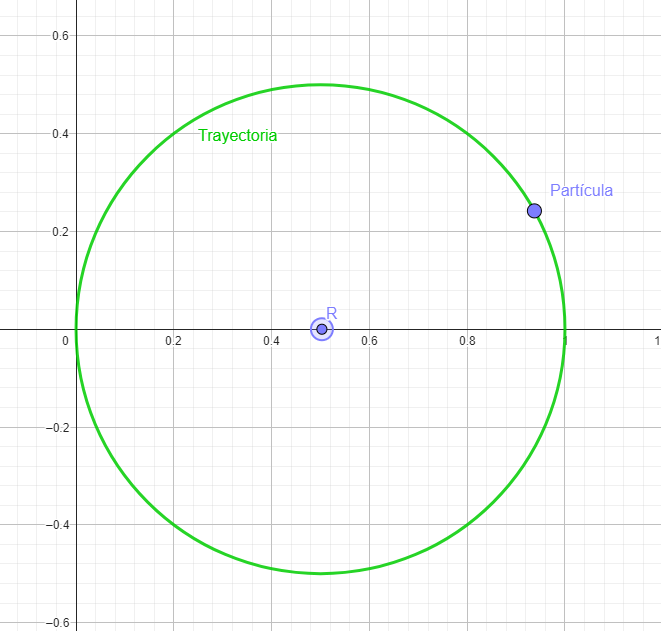
\includegraphics[width=0.5\textwidth]{Imagenes/Captura de pantalla 2024-11-29 113246.png}
\caption{Descripción de la imagen}
\label{fig:ejemplo_imagen}
\end{figure}

pongamos mas texto porque si xd, la imagen se desfasa 